% coding:utf-8

%----------------------------------------
%FOSAMATH, a LaTeX-Code for a mathematical summary for basic analysis
%Copyright (C) 2013, Daniel Winz, Ervin Mazlagic, Adrian Imboden, Philipp Langer

%This program is free software; you can redistribute it and/or
%modify it under the terms of the GNU General Public License
%as published by the Free Software Foundation; either version 2
%of the License, or (at your option) any later version.

%This program is distributed in the hope that it will be useful,
%but WITHOUT ANY WARRANTY; without even the implied warranty of
%MERCHANTABILITY or FITNESS FOR A PARTICULAR PURPOSE.  See the
%GNU General Public License for more details.
%----------------------------------------

% coding:utf-8
\documentclass[a4paper,10pt,fleqn]{article}

\usepackage{tech_ber_ei_layout}

\title{Technischer Bericht Schere}

\author{Daniel Winz}
\date{\today~\dtc}


\begin{document}

\maketitle

% \include{about}

\tableofcontents
\newpage

% % coding:utf-8

% coding:utf-8

\section{Basic Clock Modul +}

\subsection{Übersicht}
\begin{frame}
\frametitle{}
\framesubtitle{}
  \begin{figure}
    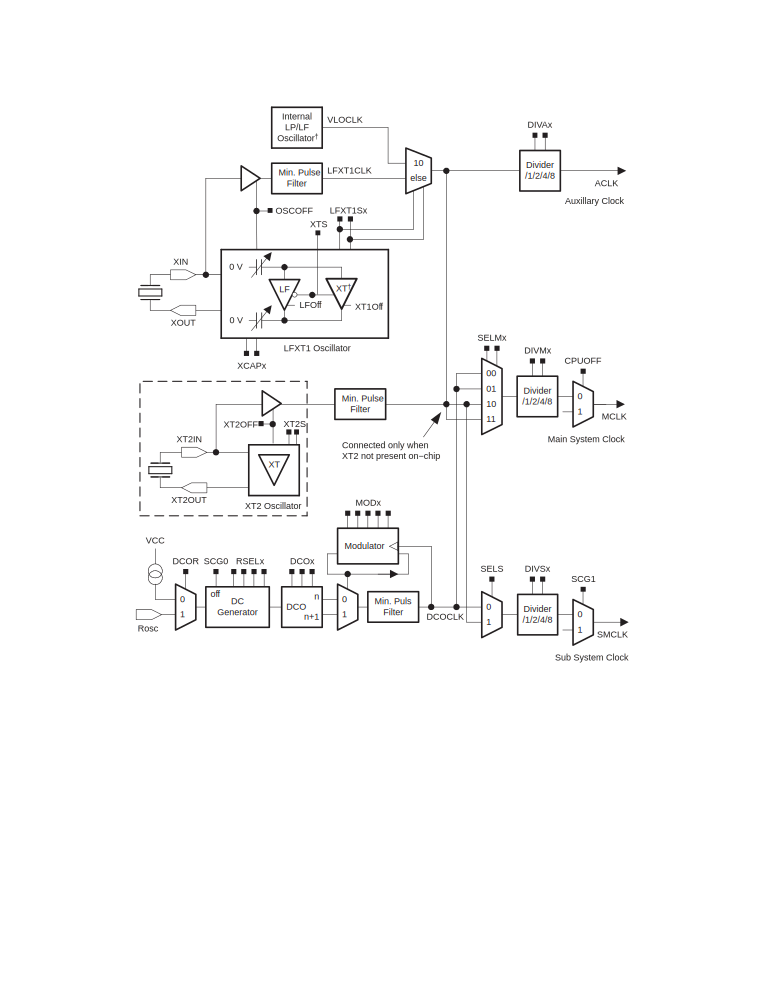
\includegraphics[width=0.5\columnwidth]{fig/ti_fg_bcm_block.pdf}
    \caption{Blockschaltbild}
  \end{figure}
\end{frame}

% \begin{frame}
% \tikzstyle{block} = [draw,fill=blue!20,text width=5em,align=center,minimum height=4em]
% \def\radius{.7mm}
% \tikzstyle{branch}=[fill,shape=circle,minimum size=3pt,inner sep=0pt]
% \begin{tikzpicture}
%   \matrix [column sep=5mm,row sep=7mm]
%   {
%     \node[block](a){a};\\
%     \node[block] (lfxt) {LF Quarzoszillator}; \&
%     \node[block] (aclk) {ACLK};
%     \\
%     \node[block] (xt)   {Quarzoszillator}; \&
%     \node[block] (mclk) {MCLK};
%     \\
%     \node[block] (dco)  {DCO}; \&
%     \node[block] (smclk){SMCLK};
%     \\
%   };
% \end{tikzpicture}
% \end{frame}

% \begin{frame}
% \begin{center}
% \tikzstyle{block} = [ draw,fill=blue!20,text width=5em,align=center,
%                       rounded corners,minimum height=3em]
% \def\radius{.7mm}
% \tikzstyle{branch}=[fill,shape=circle,minimum size=3pt,inner sep=0pt]
% \begin{tikzpicture}
%   \node[block] at (0,4) (lfxt) {LF Quarzosz.};
%   \node[block] at (5,4) (aclk) {ACLK};
%   \node[block] at (0,2) (xt)   {Quarzosz.};
%   \node[block] at (5,2) (mclk) {MCLK};
%   \node[block] at (0,0) (dco)  {DCO};
%   \node[block] at (5,0) (smclk){SMCLK};
%   \draw[-latex] (lfxt.east) -- (aclk.west);
%   \draw[-latex] (lfxt.east) -| (2.5,3) |- (mclk.west);
%   \draw[-latex] (lfxt.east) -| (2.5,2) |- (smclk.west);
%   \draw[-latex] (xt.east) -| (2.5,3) |- (aclk.west);
%   \draw[-latex] (xt.east) -- (mclk.west);
%   \draw[-latex] (xt.east) -| (2.5,2) |- (smclk.west);
%   \draw[-latex] (dco.east) -| (2.5,3) |- (aclk.west);
%   \draw[-latex] (dco.east) -| (2.5,2) |- (mclk.west);
%   \draw[-latex] (dco.east) -- (smclk.west);
% \end{tikzpicture}
% \end{center}
% \end{frame}

\begin{frame}
\begin{center}
\tikzstyle{block} = [ draw,fill=blue!20,text width=5em,align=center,
                      rounded corners,minimum height=3em]
\def\radius{.7mm}
\tikzstyle{branch}=[fill,shape=circle,minimum size=3pt,inner sep=0pt]
\begin{tikzpicture}
  \node[block] at (0,4) (lfxt) {LF Quarzosz.};
  \node[block] at (5,4) (aclk) {ACLK};
  \node[block] at (0,2) (xt)   {Quarzosz.};
  \node[block] at (5,2) (mclk) {MCLK};
  \node[block] at (0,0) (dco)  {DCO};
  \node[block] at (5,0) (smclk){SMCLK};
  \uncover<2->{\draw (0,0) node[ellipse,thick,draw=red,minimum height=2cm,
                                minimum width=3cm,draw] {};}
  \draw[-latex] (lfxt.east) -- (aclk.west);
  \draw[-latex] (lfxt.east) -- (mclk.west);
  \draw[-latex,dashed] (lfxt.east) -- (smclk.west);
%   \draw[-latex,dashed] (xt.east) -- (aclk.west);
  \draw[-latex] (xt.east) -- (mclk.west);
  \draw[-latex] (xt.east) -- (smclk.west);
%   \draw[-latex] (dco.east) -- (aclk.west);
  \draw[-latex] (dco.east) -- (mclk.west);
  \draw[-latex] (dco.east) -- (smclk.west);
\end{tikzpicture}
\end{center}
\end{frame}


% \begin{frame}
% \tikzstyle{block} = [draw, rectangle, minimum height=2em, minimum width=4em] %fill=blue!20
% \tikzstyle{sum} = [draw, fill=blue!20, circle, node distance=1cm]
% \tikzstyle{input} = [coordinate] \tikzstyle{output} = [coordinate]
% \tikzstyle{pinstyle} = [pin edge={to-,thin,black}]
% \begin{tikzpicture}[auto, node distance=2cm,>=latex’]
% \node [input, name=input] {};
% \node [sum, right of=input] (sum) {};
% \node [block, right of=sum, node distance=3.5cm] (controller) {$C(z^{-1})$};
% \node [block, right of=controller, pin={[pinstyle]above:$d(k)$}, node distance=4cm] (system) {$P(z^{-1})$};
% \draw [->] (controller) – node[name=u] {$u(k)$} (system);
% \node [output, right of=system] (output) {};
% \node [block, below of=u] (measurements) {$F(z^{-1})$};
% \draw [draw,->] (input) – node {$r(k)$} (sum);
% \draw [->] (sum) – node {$e(k)$} (controller);
% \draw [->] (system) – node [name=y] {$y(k)$}(output);
% \draw [->] (y) |- (measurements);
% \draw [->] (measurements) -| node[pos=0.99] {$-$} node [near end] {$y_m(k)$} (sum);
% \end{tikzpicture}%
%
%
%   \begin{tikzpicture}
%     [auto,
%       decision/.style={ diamond, draw=blue, thick, fill=blue!20,
%                         text width=4.5em,align=flush center,
%                         inner sep=1pt},
%       block/.style ={ rectangle, draw=blue, thick, fill=blue!20,
%                       text width=5em,align=center, rounded corners,
%                       minimum height=4em},
%       line/.style ={draw, thick, -latex',shorten >=2pt},
%       cloud/.style ={ rectangle, draw=red, thick, fill=red!20,
%                       minimum height=2em}]
%     \matrix %[column sep=5mm,row sep=7mm]
%     {
%       % row 1
%         \node [cloud] (expert) {expert}; &
%         \node [block] (init) {initialize model}; &
%         \node [cloud] (system) {system}; \\
%       % row 2
%         & \node [block] (identify) {identify candidate model}; & \\
%       % row 3
%         \node [block] (update) {update model}; &
%         \node [block] (evaluate) {evaluate candidate models}; & \\
%       % row 4
%         & \node [decision] (decide) {is best candidate}; & \\
%       % row 5
%         & \node [block] (stop) {stop}; & \\
%     };
%     \begin{scope}[every path/.style=line]
%       \path (init) -- (identify);
%       \path (identify) -- (evaluate);
%       \path (evaluate) -- (decide);
%       \path (update) |- (identify);
%       \path (decide) -| node [near start] {yes} (update);
%       \path (decide) -- node [midway] {no} (stop);
%       \path [dashed] (expert) -- (init);
%       \path [dashed] (system) -- (init);
%       \path [dashed] (system) |- (evaluate);
%     \end{scope}
%   \end{tikzpicture}
% \end{frame}                             % Basic Clock Module
% coding:utf-8

\section{Digitally-Controlled Oscillator}

\subsection{Übersicht}
\begin{frame}
    \frametitle{}
    \framesubtitle{}
      \begin{figure}
        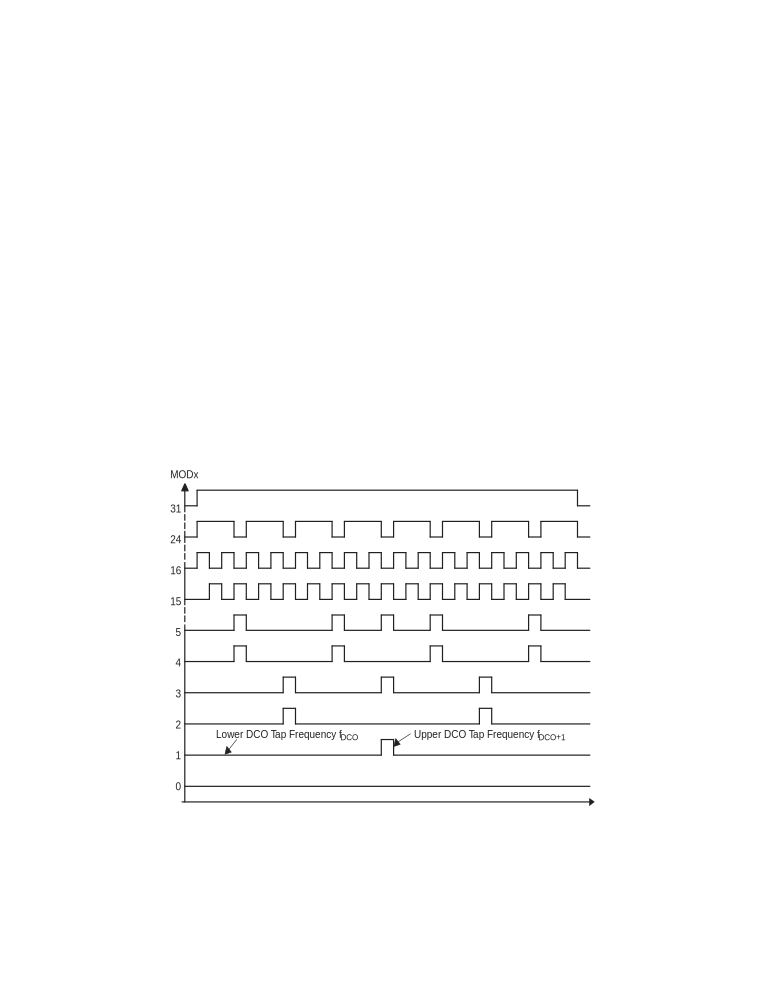
\includegraphics[width=0.7\columnwidth]{fig/ti_fg_dco_mod.pdf}
        \caption{Funktionsweise Modulation}
      \end{figure}
\end{frame}

\subsection{Modulation}
\begin{frame}
  \begin{tikztimingtable}
    \mbox{\uncover<+->{MOD =  0}} & <.->33L<*>\\
    \mbox{\uncover<+->{MOD =  1}} & <.->16LH16L<*>\\
    \mbox{\uncover<+->{MOD =  2}} & <.->8LH15LH8L<*>\\
    \mbox{\uncover<+->{MOD =  3}} & <.->8L2{H7L}H8L<*>\\
    \mbox{\uncover<+->{MOD = 16}} & <.->L16{HL}<*>\\
    \mbox{\uncover<+->{MOD = 24}} & <.->L8{3HL}<*>\\
    \mbox{\uncover<+->{MOD = 31}} & <.->L31HL<*>\\
  \end{tikztimingtable}
\end{frame}                             % Digitally-Controlled Oscillator

% \section{Basic Clock Module +}
% \subsection{Übersicht}
% \begin{frame}
%   \frametitle{Ft}
%   \begin{block}{Bt}
%     Funktionsweise des DCO
%   \end{block}
% \end{frame}
\section{Ausgangslage}
Am 15. März 2013 erhalten die Teilnehmer des Moduls Kontext 2 aus dem Bereich 
Elektrotechnik die Aufgabe, eine Vorichtung zu entwickeln, die ein Ei beim Fall 
aus einer Höhe von eineinhalb Metern schützt. Zudem muss das Ei, falls es an 
obiger Vorrichtung befestigt wird, innert nützlicher Frist aus der Vorrichtung 
herausgelöst werden können. Als Material stehen jeder Gruppe 30 Trinkhalme und 
eine Rolle Klebeband zur Verfügung. 
\cite{barmet:aufgabenstellung}

\section{Konzept}
\subsection{Trichter}
Das erste Konzept der Gruppe zwei sieht vor, dass das Ei von einem am Boden 
stehenden Trichter aufgefangen wird. Dieser Trichter soll aus Trinkhalmen 
aufgebaut werden. Dazu werden die Trinkhalme am Gelenk mittels Klebeband an 
ihrem Gelenk zusammengebunden. die langen Enden werden dabei zu einem Trichter 
aufgefächert. Die kurzen Enden werden abgespreizt und dienen somit als 
Standfuss. 

\subsubsection*{Vorteile}
\begin{itemize}
  \item Die Schutzwirkung ist unabhängig davon, in welcher Lage das Ei am Boden 
        ankommt. 
  \item einfacher Aufbau
\end{itemize}

\subsubsection*{Nachteile}
\begin{itemize}
  \item Die Schutzwirkung ist abhängig davon, ob der Trichter getroffen wird. 
  \item Befestigung des Trichters am Boden könnte problematisch sein. 
\end{itemize}

\subsection{"'Airbag"'}
Das zweite Konzept sieht vor, dass das Ei in der Schutzvorrichtung befestigt 
wird. Dazu werden zwei Trichter wie beim vorhergehenden Konzept hergestellt. 
Das Ei wird zwischen den Trichtern Platziert. Anschliessend werden die 
Trichter ineinander geschoben. 

\subsubsection*{Vorteile}
\begin{itemize}
  \item Die Schutzwirkung ist nicht davon abhängig, ob die Schutzvorrichtung 
        getroffen wird. 
\end{itemize}

\subsubsection*{Nachteile}
\begin{itemize}
  \item Die Lage beim Aufprall ist nicht unerheblich für die Schutzwirkung. 
  \item Der Aufbau ist komplexer als 
\end{itemize}




\section{Schlussfolgerungen}

\bibliographystyle{apacite}
\bibliography{tech_ber_ei}{}

\end{document}

